\section{Three nervous systems and one plan}\label{sec:brains}

The selector of Section~\ref{ssec:selector} borrows three mechanisms from nervous systems: a race to threshold, a reward that potentiates the winner, and homeostatic scaling. This section shows where the rest of the architecture of a BLLM sits in the wiring of real brains. We use three complete reconstructions: the nervous system of the nematode \textit{Caenorhabditis elegans} \cite{CJB19}, the whole brain of the adult fruit fly \textit{Drosophila melanogaster} \cite{DMS24b}, and a cubic millimetre of human temporal cortex \cite{SJB24}.\footnote{The worm is the hermaphrodite of S.~J. Cook et al., Nature 571 (2019) 63--71 \cite{CJB19}, in the edge list distributed by the OpenWorm project, with the classes of sensory and motor neurons of L.~R. Varshney et al. \cite{VCP11}. The fly is FlyWire, S.~Dorkenwald et al., Nature 634 (2024) 124--138 \cite{DMS24b}, release 783 of the proofread connections (Zenodo, doi:10.5281/zenodo.10676866, CC BY 4.0), with the transmitters predicted from electron micrographs by N.~Eckstein et al. \cite{EBC24}. The cortex is H01, A.~Shapson-Coe et al., Science 384 (2024) eadk4858 \cite{SJB24}, in its table of somas. The files are public and are not redistributed; the BLLM package reads them from the paths a user gives, and the summaries behind Figs.~\ref{fig:worm} to~\ref{fig:cortex} are computed by a program in the repository of the paper.} In each of them the same plan appears: signals enter at one end, are integrated in a middle stage that is mostly recurrent, and leave at the other end, with feedback from the output back to the input (Fig.~\ref{fig:brainmap}(a)). A BLLM has the same plan with a different meaning of each stage (Fig.~\ref{fig:brainmap}(b)): the proposers sense, the selector integrates, the checks act, and the memory feeds back.

\begin{figure*}[t]
\centering
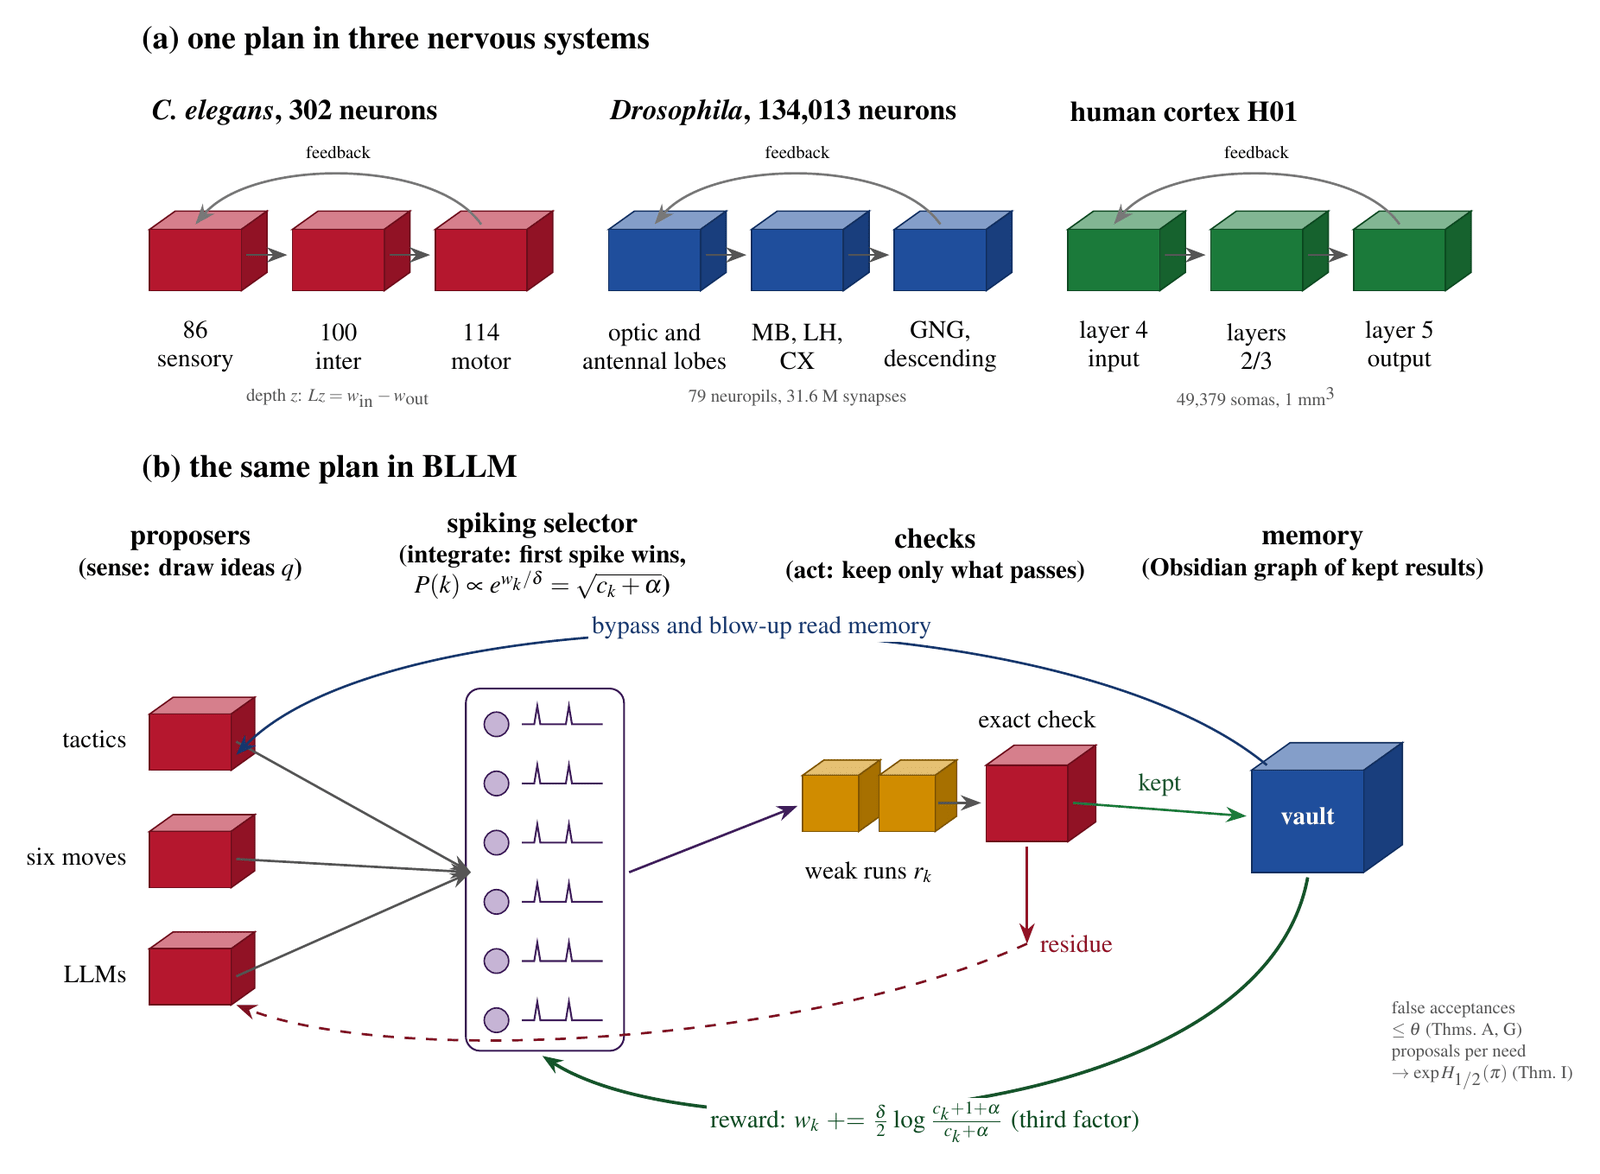
\includegraphics[width=0.98\textwidth]{figures/fig_brainmap}
\caption{One plan in three nervous systems and in a BLLM. (a) Sensory, integrating and output stages, with feedback, in the worm \cite{CJB19}, the fly \cite{DMS24b} and the human cortex \cite{SJB24}; the numbers are those of the reconstructions. (b) The same plan in a BLLM: proposers (language models, the six moves of Section~\ref{ssec:moves}, tactic search) draw ideas from a profile $q$; the spiking selector of Section~\ref{ssec:selector} chooses who proposes next by a race to the first spike; weak runs and one exact check keep only what passes (Theorem~\ref{thm:cascade}); kept results enter the memory, which bypass and blow-up read, and send the reward \eqref{eq:spikereward} back to the selector; rejected candidates leave residues for the proposers. The checks bound the expected number of false acceptances by $\theta$ (Theorems~\ref{thm:A} and~\ref{thm:G}), and the selector brings the number of proposals per need to $e^{H_{1/2}(\pi)}$ (Theorem~\ref{thm:I}).}
\label{fig:brainmap}
\end{figure*}

\subsection{The worm: depth of processing}

The hermaphrodite connectome has $448$ nodes, $300$ neurons and $148$ muscles and end organs, with $27{,}019$ chemical synapses in $4{,}681$ connections and $12{,}683$ gap-junction contacts in $2{,}698$. Varshney and coauthors gave its neurons a \emph{processing depth} \cite{VCP11}: a coordinate that increases along the direction in which signals travel. Let $W$ be the matrix of synaptic weights, $\mathrm{in}_{k}=\sum_{i}W_{ik}$ and $\mathrm{out}_{k}=\sum_{j}W_{kj}$, and let $L$ be the Laplacian of the symmetric matrix $(W+W^{\top})/2$.

\begin{lemma}[Processing depth]\label{lem:depth}
The system $Lz=\mathrm{in}-\mathrm{out}$ has a solution, unique up to an additive constant on each connected component, and it is the minimiser of $\sum_{i,j}W_{ij}(z_{j}-z_{i}-2)^{2}$.
\end{lemma}

\begin{proof}
The kernel of $L$ is spanned by the indicator vectors of the connected components, and $L$ is symmetric, so its range is the set of vectors that sum to zero on every component. Each synapse $i\to j$ adds $W_{ij}$ to $\mathrm{in}_{j}$ and to $\mathrm{out}_{i}$, both in the same component, so $\mathrm{in}-\mathrm{out}$ sums to zero there. For the variational form, $z^{\top}Lz=\frac12\sum_{i,j}W_{ij}(z_{j}-z_{i})^{2}$ and $(\mathrm{in}-\mathrm{out})^{\top}z=\sum_{i,j}W_{ij}(z_{j}-z_{i})$, so $\frac12z^{\top}Lz-(\mathrm{in}-\mathrm{out})^{\top}z=\frac14\sum_{i,j}W_{ij}(z_{j}-z_{i}-2)^{2}-\sum_{i,j}W_{ij}$, a convex function whose critical points are the solutions.
\end{proof}

So $z$ is the arrangement in which every synapse comes as close as possible to pointing two units deeper; with another normalisation of the Laplacian the unit changes and the order does not. Computed on the chemical and electrical synapses together, the mean depth is $-1.92$ for the $86$ sensory neurons, $-0.68$ for the $100$ interneurons, $-0.22$ for the $114$ motor neurons and $+1.75$ for the muscles. Four of the five shallowest neurons are amphid sensory neurons, AWAL, AWAR, ASIL and ASEL, and the deepest nodes are pharyngeal muscles and marginal cells. The order sensory, inter, motor, muscle is not imposed; it is computed from the wiring alone, and it is the order of the three stages of Fig.~\ref{fig:brainmap}(a). Figure~\ref{fig:worm} draws every node at its depth, against a spectral coordinate: the rank of the node in the lowest eigenvector of the normalised Laplacian that is spread over at least a quarter of the neurons, the third, with eigenvalue $0.123$.

\begin{figure*}[t]
\centering
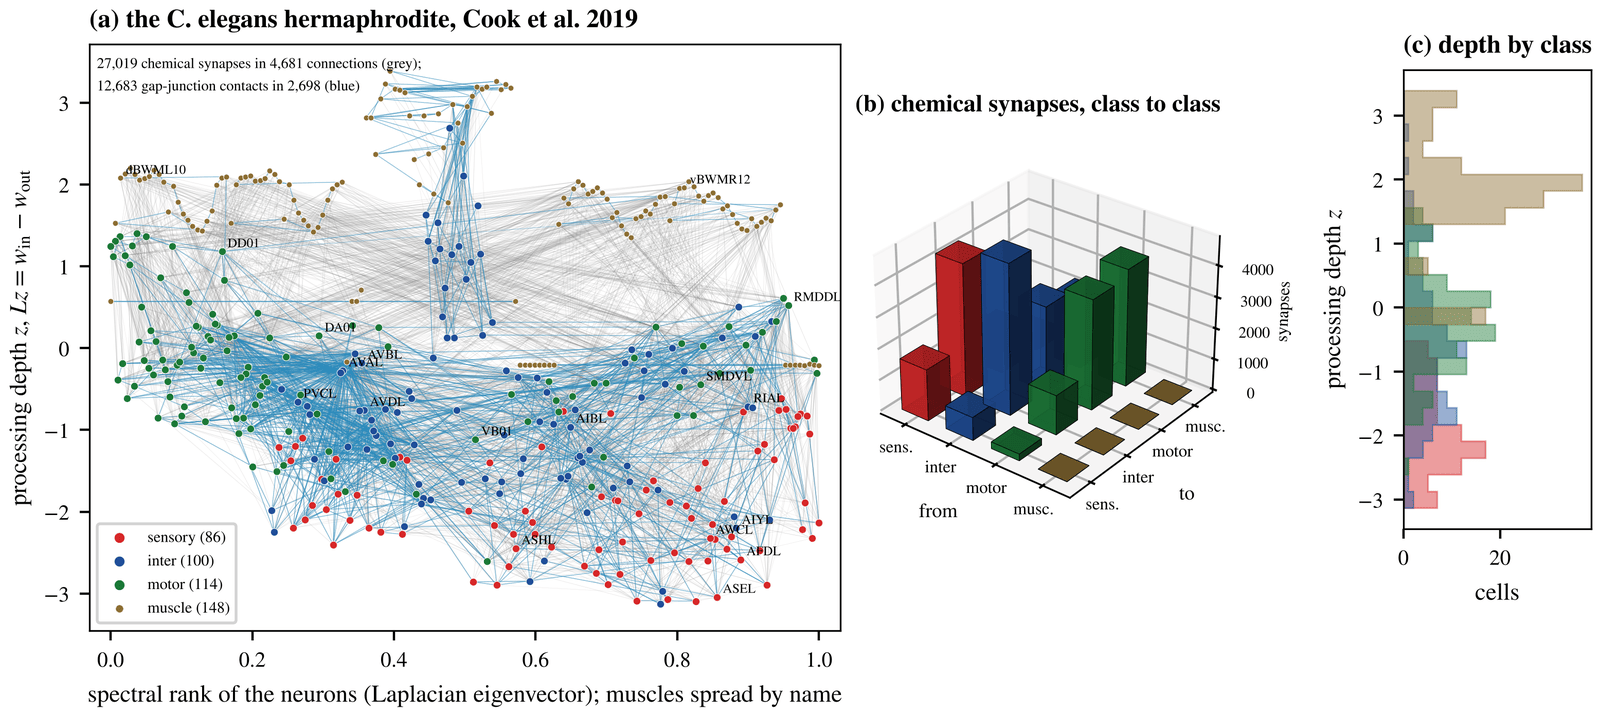
\includegraphics[width=0.98\textwidth]{figures/fig_worm}
\caption{The \textit{C.~elegans} hermaphrodite \cite{CJB19}. (a) Every neuron and muscle at its processing depth $z$ (Lemma~\ref{lem:depth}) against its rank in a spectral coordinate of the neurons, with chemical connections in grey and gap junctions in blue; muscles, which have no spectral coordinate, are spread by name. Sensory neurons lie lowest and muscles highest. (b) Chemical synapses from class to class: the largest flows are from sensory neurons to interneurons, from interneurons to interneurons and motor neurons, and from motor neurons to muscles. (c) The distribution of depths in each class.}
\label{fig:worm}
\end{figure*}

The package can also run this wiring. It builds an echo-state network whose recurrent matrix is the connectome itself, scaled to spectral radius $0.9$, with one sign per presynaptic neuron, as Dale's principle requires (excitatory with probability $0.8$, since the transmitter map of the worm is not part of the wiring data), and fits a linear readout \cite{JH04}. Its short-term memory, the squared correlation between the input $k$ steps back and its best linear readout from sixty units, is $0.77$, $0.37$, $0.27$ and $0.14$ for $k=1,2,4,8$. This makes no claim that a worm-shaped reservoir computes better than another; it lets the memory and the selector of a BLLM be wired as a real circuit, which is what the experiments of Lappalainen and coauthors show to be informative in the fly, where networks constrained by the connectome predict the activity of the visual system neuron by neuron \cite{LTP24}.

\subsection{The fly: 79 neuropils}

At a threshold of five synapses per connection the FlyWire brain has $134{,}013$ neurons, $2{,}710{,}038$ connections and $31{,}578{,}726$ synapses in $79$ neuropils. Give each neuron the neuropil where it receives most of its input, and count every synapse from the neuropil of its presynaptic neuron to the neuropil where it lies. The resulting matrix (Fig.~\ref{fig:fly}(a)) has $59.0\%$ of its weight on the diagonal: most synapses are made where the presynaptic neuron itself listens, a local and recurrent integration. The off-diagonal weight connects the stages of Fig.~\ref{fig:brainmap}(a): the optic lobes and antennal lobes, which receive the senses, project to the mushroom bodies, the lateral horn and the central complex, which integrate and learn, and these to the premotor neuropils and the gnathal ganglion, where the descending neurons leave for the body. Acetylcholine, excitatory in the fly, is the predicted transmitter of $57.1\%$ of the synapses, GABA of $24.7\%$ and glutamate, mostly inhibitory, of $16.4\%$; serotonin, dopamine and octopamine together of $1.8\%$, concentrated in the mushroom bodies where dopamine carries the reward signal of associative learning. The numbers of partners are heavy-tailed: the median neuron has $11$ output partners and $10$ input partners, the mean about $19$, and the largest $6{,}398$ and $5{,}066$ (Fig.~\ref{fig:fly}(c)).

\begin{figure*}[t]
\centering
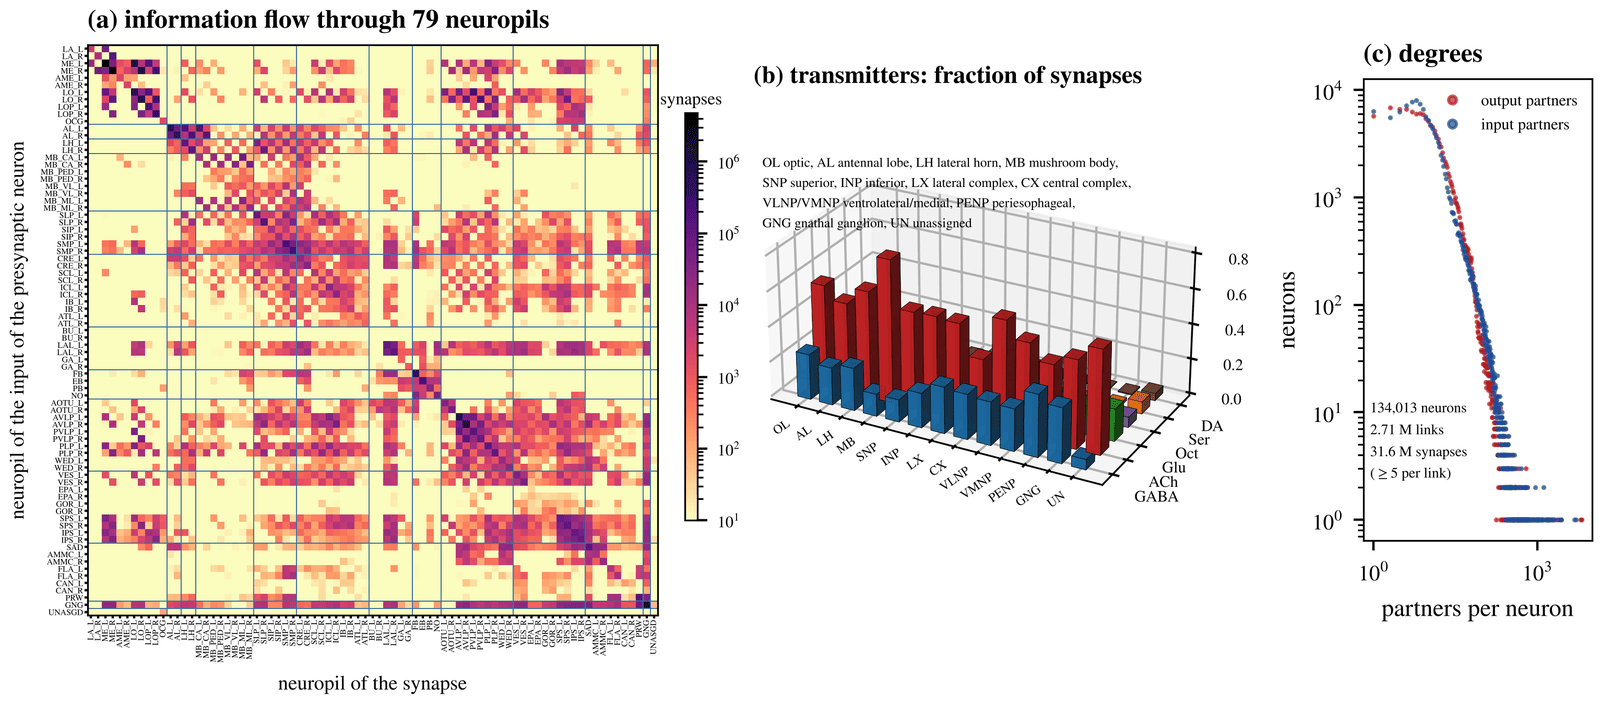
\includegraphics[width=0.98\textwidth]{figures/fig_fly}
\caption{The adult \textit{Drosophila} brain, FlyWire release 783, connections of at least five synapses \cite{DMS24b}. (a) Synapses from the neuropil where the presynaptic neuron receives most of its input (rows) to the neuropil of the synapse (columns), on a logarithmic scale, with the neuropils grouped into the super-groups of FlyWire; $59\%$ of the weight is on the diagonal. (b) The predicted transmitter of the synapses \cite{EBC24} in each super-group. (c) The numbers of output and input partners per neuron.}
\label{fig:fly}
\end{figure*}

\subsection{The human cortex: six layers}

H01 is a fragment of human temporal cortex of about a cubic millimetre, reconstructed by electron microscopy at nanometre resolution \cite{SJB24}. Its table of somas lists $49{,}379$ cells: $20{,}139$ oligodendrocytes, $8{,}803$ pyramidal neurons, $6{,}536$ microglia and precursor cells, $5{,}474$ astrocytes and $4{,}688$ interneurons, among others, with $16{,}253$ neurons in all. The layers are its stages (Fig.~\ref{fig:cortex}). Layer~1 holds almost no neurons ($2\%$ of its cells are pyramidal); pyramidal neurons are $40\%$ of the cells of layer~2, $25\%$ of layer~3, $33\%$ of layer~4, $18\%$ of layer~5 and $16\%$ of layer~6, interneurons are densest in layer~2 ($24\%$), and the white matter below is $77\%$ oligodendrocytes, the insulation of the axons that leave. In the canonical circuit of the neocortex \cite{DM04}, input from the thalamus arrives in layer~4, is integrated in the recurrent networks of layers~2 and~3, and leaves from the large pyramidal neurons of layer~5, with feedback from layer~6 to the thalamus: the plan of Fig.~\ref{fig:brainmap}(a) again.

\begin{figure*}[t]
\centering
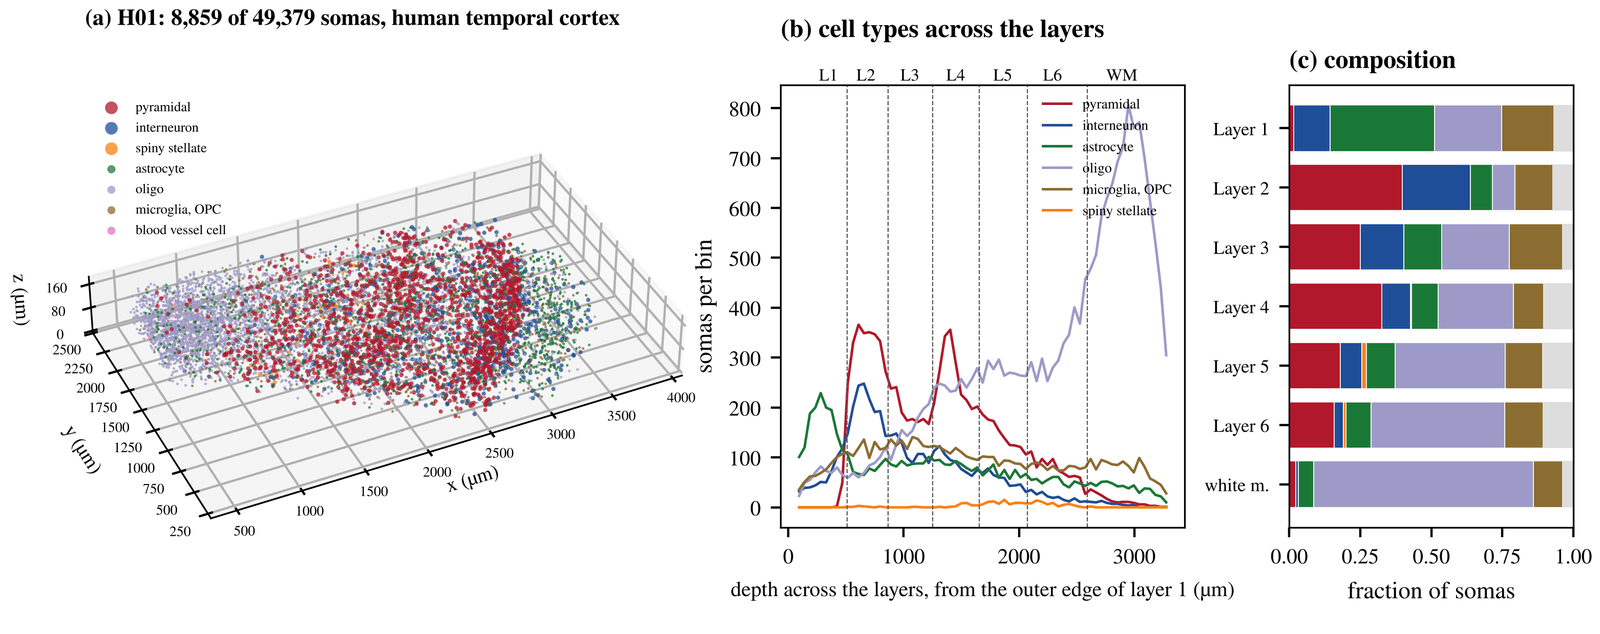
\includegraphics[width=0.98\textwidth]{figures/fig_cortex}
\caption{The human cortical fragment H01 \cite{SJB24}. (a) A random sample of $8{,}859$ of its $49{,}379$ somas at their positions, coloured by cell type. (b) The number of somas of each type along the axis of the layers, measured from the outer edge of layer~1, with the boundaries between layers. (c) The composition of each layer and of the white matter.}
\label{fig:cortex}
\end{figure*}

\subsection{From wiring to a BLLM}

The three stages carry over with a precise meaning. The \emph{sensing} stage is the set of proposers, whose profile $q$ is what Theorem~\ref{thm:I} measures. The \emph{integrating} stage is the selector, whose job, like that of the basal ganglia in the account of Redgrave, Prescott and Gurney \cite{RPG99}, is to choose one action among competing ones and to learn from a reward signal which choices pay, the role that dopamine plays in the account of Schultz, Dayan and Montague \cite{SDM97}; Proposition~\ref{prop:spiking} shows that with a race to the first spike this choice is square-root sampling, the optimum of the gap law. The \emph{acting} stage is the cascade of checks, which lets through only what passes, and the \emph{feedback} is the memory and the residues. One part of the plan of a brain has no counterpart: no stage of a nervous system certifies what it keeps, and that is the part this paper adds. A BLLM is therefore not a model of a brain. It is a system that keeps the organisation which brains share, replaces the stage that decides by a check whose cost is priced by Theorems~\ref{thm:A} to~\ref{thm:H}, and uses at the stage of choice the mechanism that the gap law shows to be optimal. Because the selector is a circuit of leaky integrate-and-fire neurons with a local learning rule, it can run on neuromorphic hardware \cite{Mea90,DSL18}; we have run it only in simulation.
